\chapter{Design}
\label{ch:design}

\begin{figure}[h]
    \center{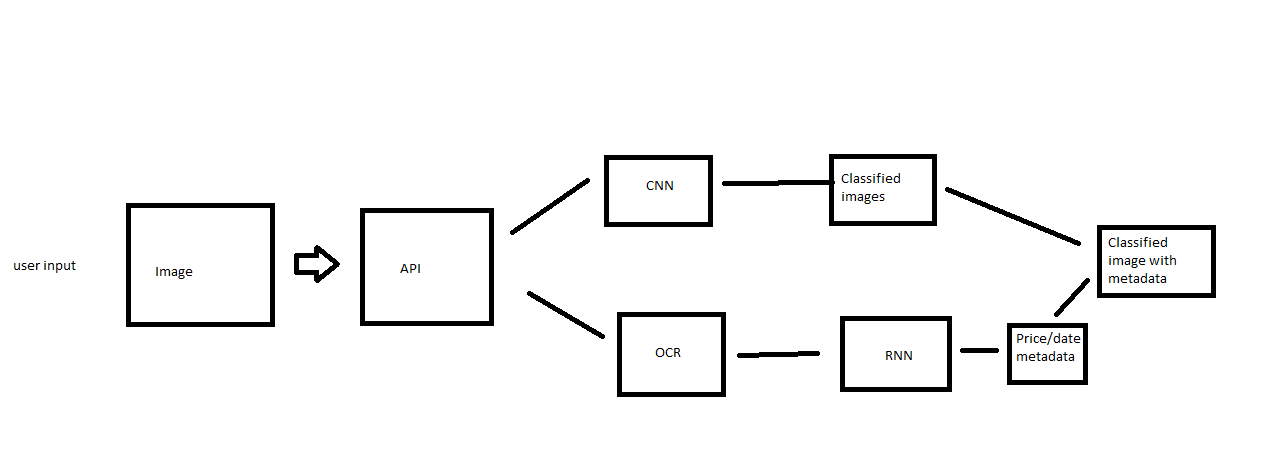
\includegraphics[width=1\textwidth]{Images/pipeline}}
    \caption{Graphic illustrating the project pipeline (PLACEHOLDER)}
    \label{fig:figure3}
\end{figure}
The project is designed to be able to take an input image of a receipt sent over http, and provide metadata to that image based on its contents.
This metadata includes the company name that issued the receipt, the date the receipt was made, and the price of the purchase.
In order to transfer the image to our machine learning models, a .NET API is used.

The API exposes several endpoints that allows for saving an image and a receipt to a database.
The API is also connected to the ML and OCR module.

We have decided to split up the metadata extraction into two separate parts;
a Convolutional Neural Network for image classification and a Recurrent Neural Network for natural language processing.

The CNN will take an image as input, and decide which company issued that receipt based on previous training data.

The RNN will take text as input.
In order to extract the text from the images, an open-source OCR is used.

Finally, the outputs of the CNN and RNN and combined and provided back to the user.
This pipeline is illustrated in figure 3.1

\section{API}\label{sec:API}
The API is used as the connection point between the different endpoints

\section{Dataset}\label{sec:dataset}
In order to train our neural network models, Simployer provided us with a sample of images from their database.
This dataset includes 1194 images of receipts taken with mobile cameras and generated pdfs from online sales.

\begin{figure}[h]
    \center{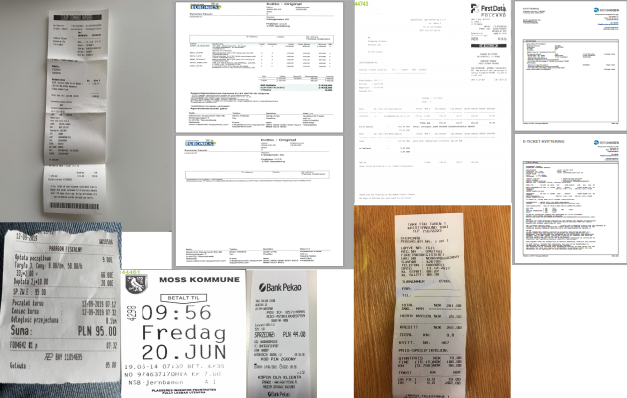
\includegraphics[width=1\textwidth]{Images/exampleimages_raw_resized}}
    \caption{Examples of the images found in the dataset provided by Simployer}
    \label{fig:figure3.2}
\end{figure}

This dataset is not labeled, which means we have to manually label the data we are going to use to train our networks.
Because of the large variance of different types of companies in this dataset, creating labels for all of them would be very time-consuming.
Instead of labeling them all, we decided to restrict ourselves to the three most common receipts found in the dataset.
This means the amount of images we can use for training is greatly reduced, so in order to combat this, we used data augmentation software to generate more images.
This is discussed in greater detail in chapter 4.

\section{Pre-processing}\label{sec:pre-processing}
A CNN does not require images of large resolution in order to accurately classify an image.
In addition, training the network with large resolution images take significantly longer.
Because of this, all the images that are going to be fed into the CNN are downscaled.
This also solves the problem of images being of different sizes, as the CNN requires all the images to have the same size.

\begin{figure}[h]
    \center{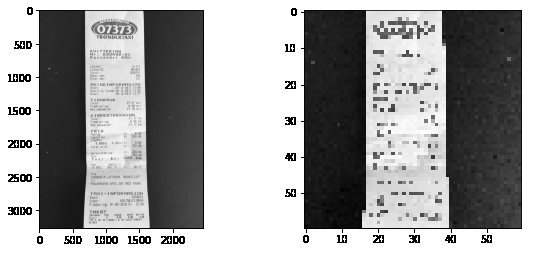
\includegraphics[width=1\textwidth]{Images/beforeafterrescale}}
    \caption{Before and after image rescaling}
    \label{fig:figure3.3}
\end{figure}
While the text in the image is now completely unreadable, the CNN will have no issues telling images in this format apart from each other.

\section{Convolutional Neural network}\label{sec:CNN}
As stated previously, we are using a CNN as an image classifier in order to determine which company issued the receipt.

\begin{figure}[h]
    \center{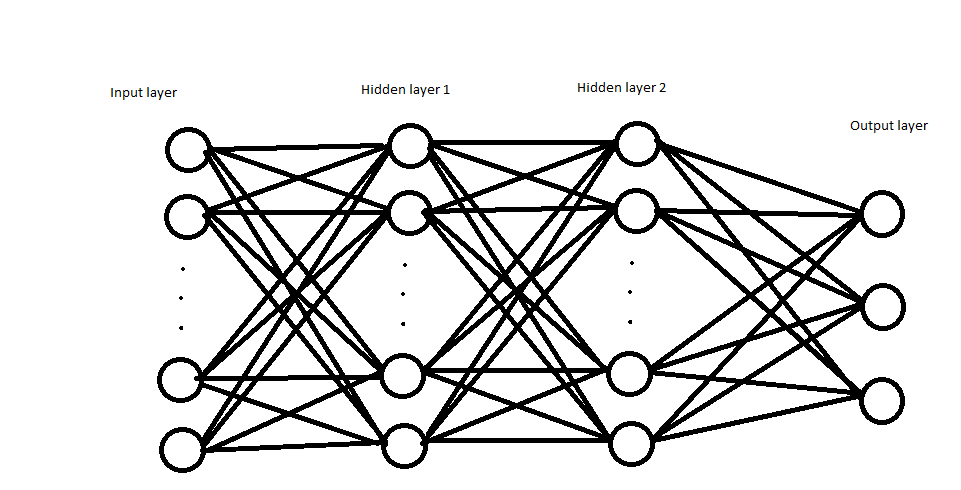
\includegraphics[width=1\textwidth]{Images/cnnplaceholder}}
    \caption{Graphic illustrating the Convolutional Neural Network (PLACEHOLDER)}
    \label{fig:figure3.4}
\end{figure}

Figure 3.3 illustrates the layout of our CNN.
The input layer takes the pixel value of the image.
Because of this, the number of nodes in the input layer has to be equal to the amount of pixels in the image.
The output layer has three nodes, one for each type of receipt the network is trained to classify.

We are using a supervised learning-model to train our network.
Because of this, the training data has to be labeled.
This labeling can be labor intensive if the dataset you are labeling is large.
Since we started with a very small amount of images before the use of data augmentation, it is a small task.

\section{Optical Character Recognition}\label{sec:OCR}
In order to extract the text found in an image, we are using the open-source OCR software Python-tesseract.
Python-tesseract, or Pytesseract for short, utilizes Google's Tesseract-OCR engine.

When metadata for a particular image is requested by a user, the API will provide our implementation of Pytesseract with an image.
Pytesseract will take this image as an input, and can provide outputs in various formats like xml or pdf.
We will be using the output in string format, as this will serve as the input to our RNN model.
Once Pytesseract has completed the text extraction, the output string is then fetched by our API to be provided to our RNN model.

\begin{figure}[h]
    \center{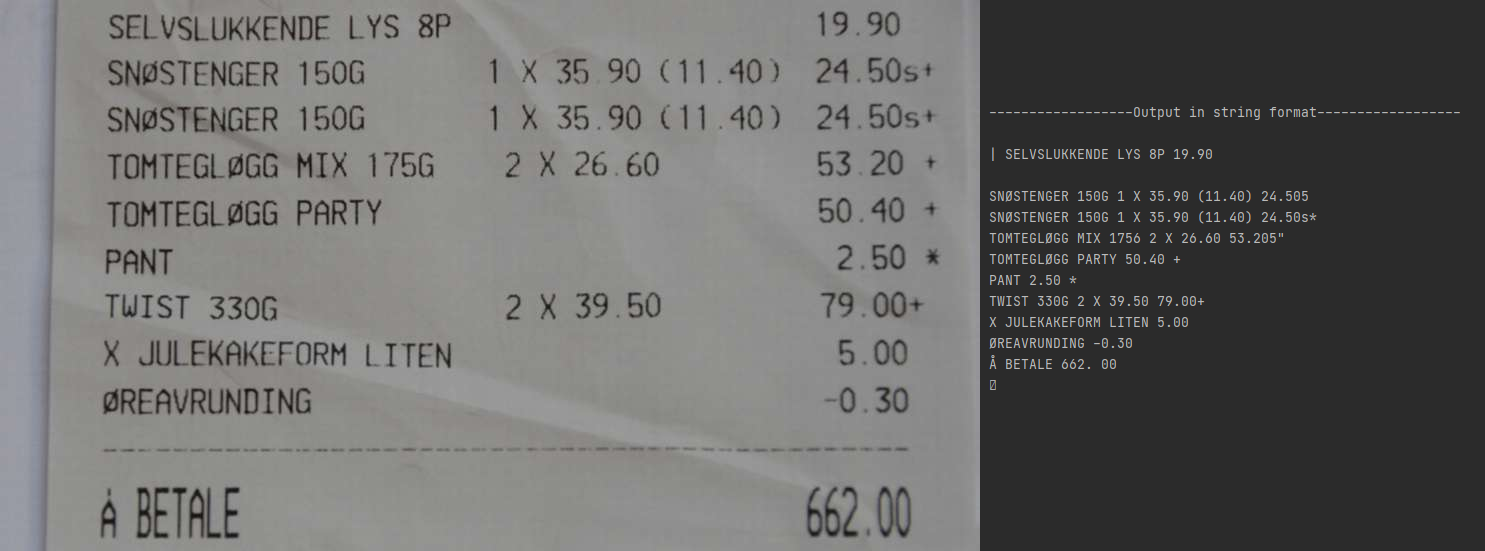
\includegraphics[width=1\textwidth]{Images/ocr_before_after}}
    \caption{Example output of pytesseract with a test image}
    \label{fig:figure3.5}
\end{figure}

\section{Recurrent Neural Network}\label{sec:RNN}

